\section{Smoothness Classes}\label{sec:smoothness}

The regression function $m(x,z)$ is a bivariate function whose smoothness can be formalized in several ways.
This section defines the anisotropic Lipschitz class, which is the maintained smoothness assumption throughout the paper.
An alternative isotropic (joint) smoothness class and its relationship to the anisotropic class are discussed in \cref{sec:appendix:isotropic}.

Throughout, I focus on order $p = 1$ (Lipschitz continuity), which governs the worst-case bias of the local constant estimator.


\subsection{Anisotropic Smoothness}\label{sec:smoothness:anisotropic}

The anisotropic class allows independent control of smoothness in each coordinate direction.

\begin{definition}[Anisotropic Lipschitz Class]\label{def:anisotropic}
	The anisotropic Lipschitz class with constants $M_x, M_z > 0$ is
	\begin{equation}\label{eq:anisotropic}
		\mathcal{F}_1^{\mathrm{aniso}}(M_x, M_z) \defeq \bigl\{ f : \mathbb{R}^2 \to \mathbb{R} \;\big|\; \abs{f(x,z) - f(x',z)} \leq M_x\abs{x - x'} \;\forall\, z, \;\; \abs{f(x,z) - f(x,z')} \leq M_z\abs{z - z'} \;\forall\, x \bigr\}.
	\end{equation}
\end{definition}

This directly bounds each partial derivative independently: $\abs{\partial f / \partial x} \leq M_x$ and $\abs{\partial f / \partial z} \leq M_z$, with no coupling between the two.
\Cref{fig:smoothness_classes} illustrates the feasible gradient sets for both the anisotropic and isotropic classes when $M_x = M_z = M$.

\begin{figure}[ht]
\centering
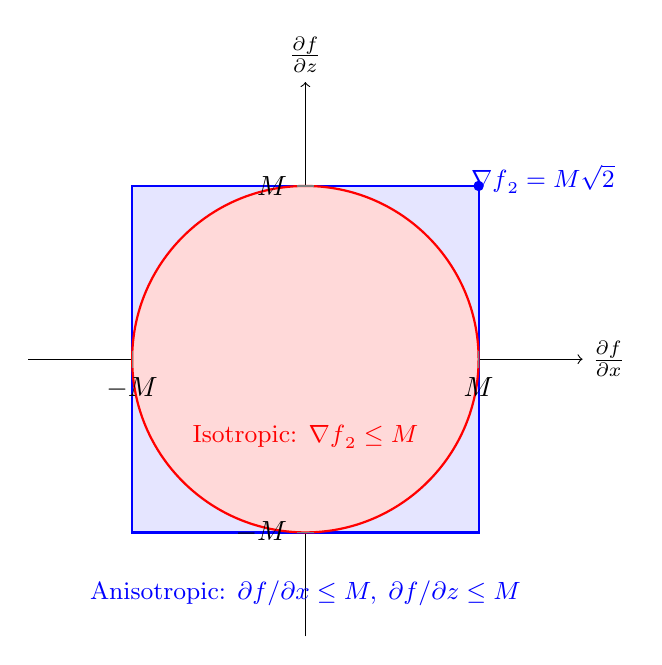
\begin{tikzpicture}[scale=2.2]
	% Axes
	\draw[->] (-1.6,0) -- (1.6,0) node[right] {$\frac{\partial f}{\partial x}$};
	\draw[->] (0,-1.6) -- (0,1.6) node[above] {$\frac{\partial f}{\partial z}$};

	% Anisotropic square (M_x = M_z = M)
	\fill[blue!10, draw=blue, thick]
		(-1,-1) rectangle (1,1);

	% Isotropic disk
	\fill[red!15, draw=red, thick]
		(0,0) circle (1);

	% Labels for M on axes
	\draw[thin, gray] (1,0.05) -- (1,-0.05) node[below, black] {$M$};
	\draw[thin, gray] (-1,0.05) -- (-1,-0.05) node[below, black] {$-M$};
	\draw[thin, gray] (0.05,1) -- (-0.05,1) node[left, black] {$M$};
	\draw[thin, gray] (0.05,-1) -- (-0.05,-1) node[left, black] {$-M$};

	% Corner point of square not in disk
	\fill[blue] (1,1) circle (0.03);
	\node[blue, above right, font=\small] at (0.9,0.9) {$\norm{\nabla f}_2 = M\sqrt{2}$};

	% Legend
	\node[red, font=\small] at (0, -0.45) {Isotropic: $\norm{\nabla f}_2 \leq M$};
	\node[blue, font=\small] at (0, -1.35) {Anisotropic: $\abs{\partial f/\partial x} \leq M,\; \abs{\partial f/\partial z} \leq M$};
\end{tikzpicture}
\caption{Feasible gradient sets for the isotropic and anisotropic Lipschitz classes with equal constants $M_x = M_z = M$.
The isotropic class constrains the gradient to lie in the disk (red); the anisotropic class constrains it to the square (blue).
The square strictly contains the disk: $\mathcal{F}_1^{\mathrm{iso}}(M) \subsetneq \mathcal{F}_1^{\mathrm{aniso}}(M, M)$.
At the corner $(M, M)$, the gradient magnitude is $M\sqrt{2}$, so a function with both partial derivatives at their bound lies in the anisotropic class but not the isotropic class.}
\label{fig:smoothness_classes}
\end{figure}


\paragraph{Directional derivatives.}
The anisotropic class also controls movement in arbitrary directions.
For a unit vector $\vec{v} = (v_1, v_2)$ and step size $t > 0$:
\begin{align}
	\abs{f(x + tv_1,\, z + tv_2) - f(x, z)}
	&\leq \abs{f(x + tv_1,\, z + tv_2) - f(x,\, z + tv_2)} + \abs{f(x,\, z + tv_2) - f(x, z)} \nonumber\\
	&\leq M_x \abs{tv_1} + M_z \abs{tv_2}. \label{eq:aniso_directional}
\end{align}
The directional derivative along $\vec{v}$ is therefore bounded by $M_x\abs{v_1} + M_z\abs{v_2}$.
This bound is direction-dependent but always finite.
The worst-case direction, found by maximizing over unit vectors via Cauchy--Schwarz, gives:
\begin{equation}\label{eq:aniso_worst_direction}
	\sup_{\norm{\vec{v}}_2 = 1} \bigl(M_x\abs{v_1} + M_z\abs{v_2}\bigr) = \sqrt{M_x^2 + M_z^2},
\end{equation}
achieved at $\vec{v}^* \propto (M_x, M_z)$.


\subsection{Why the Anisotropic Class}\label{sec:smoothness:discussion}

The anisotropic class is not merely a technical convenience --- it is the weakest smoothness class under which covariate adjustment via segmentation yields a strict improvement in worst-case bias.

\paragraph{Fungibility under isotropic smoothness.}
The isotropic class $\mathcal{F}_1^{\mathrm{iso}}(M)$ requires $\norm{\nabla f}_2 \leq M$, constraining the gradient to lie in a disk of radius $M$ (\cref{sec:appendix:isotropic}).
This couples the partial derivatives: $(\partial f / \partial x)^2 + (\partial f / \partial z)^2 \leq M^2$.
The curvature budget is therefore \emph{fungible} across directions.
If an estimator controls for the $z$-direction --- as segmentation does by restricting comparisons to narrow segments --- the worst-case function reallocates its entire curvature budget to the $x$-direction, setting $\partial f / \partial z = 0$ and $\partial f / \partial x = M$.
The worst-case bias remains $h \cdot M \cdot B_{1,0}$, identical to the pooled estimator.
Under the isotropic class, segmentation cannot reduce worst-case bias.

\paragraph{Separated budgets under anisotropic smoothness.}
The anisotropic class bounds $\abs{\partial f / \partial x} \leq M_x$ and $\abs{\partial f / \partial z} \leq M_z$ independently.
The $M_z$ budget cannot be redirected into the $x$-direction.
When segmentation neutralizes the $z$-channel of the bias, the $M_z$ budget is stranded: it can only generate within-segment compositional variation proportional to $M_z \cdot \delta$, which vanishes as the segment width $\delta \to 0$.
The worst-case bias of the segmented estimator therefore depends primarily on $M_x$, yielding a strict improvement over the pooled estimator whenever $M_z > 0$ and $\delta$ is sufficiently small.

\paragraph{Geographic interpretation.}
In geographic RD settings, the anisotropic class captures a natural assumption: the regression function has a fixed smoothness structure that does not respond to the researcher's estimation choices.
The isotropic class, by contrast, has a counterintuitive implication.
As the bandwidth $h$ shrinks (restricting attention to units closer to the boundary), the estimator becomes less sensitive to $x$-variation.
Under the isotropic constraint, the worst-case function exploits this by shifting curvature from $x$ into $z$ --- effectively becoming more curved \emph{along the boundary} as the researcher zooms in closer to it.
There is no substantive reason to expect this in geographic applications: the smoothness of outcomes along the boundary should not depend on how the researcher chooses to estimate.
The anisotropic class avoids this by fixing $M_x$ and $M_z$ independently of the bandwidth.

\paragraph{Nesting.}
The anisotropic class is strictly weaker than the isotropic class: $\mathcal{F}_1^{\mathrm{iso}}(M) \subsetneq \mathcal{F}_1^{\mathrm{aniso}}(M, M)$.
Results established under $\mathcal{F}_1^{\mathrm{aniso}}(M_x, M_z)$ therefore remain valid if the data-generating process satisfies isotropic smoothness --- in that case the anisotropic bounds are conservative but not misleading.
Setting $M_x = M_z$ corresponds to the belief that the regression function varies equally smoothly in both directions without imposing the additional coupling constraint of the isotropic class.
